\documentclass[letterpaper]{article}
\usepackage{iftex}
\ifPDFTeX
  % Submission path: use the unmodified official AAAI style with PDFLaTeX.
  \makeatletter
  \def\input@path{{../../../EGO_paper/EGO_AAAI27/}}
  \makeatother
  \usepackage[submission]{aaai2027}
\else
  % Portable preview path for Tectonic/XeTeX in environments without PDFLaTeX.
  % It mirrors the AAAI page and column geometry but is not a submission build.
  \usepackage[margin=0.75in,columnsep=0.375in]{geometry}
  \usepackage{authblk}
  \setlength{\affilsep}{0pt}
  \twocolumn
\fi
\usepackage[hyphens]{url}
\usepackage{graphicx}
\urlstyle{rm}
\def\UrlFont{\rm}
\usepackage{natbib}
\usepackage{caption}
\frenchspacing

\usepackage{booktabs}
\usepackage{amsmath}
\usepackage{amssymb}
\usepackage{xcolor}
\usepackage{tikz}

% DRAFT COLOR CONTRACT:
%   blue = measured value; red = preregistered claim rejected by the final result.
% Before submission, resolve the red claim in prose and redefine both macros
% as identity functions.
\definecolor{measuredblue}{RGB}{0,73,160}
\definecolor{pendingred}{RGB}{190,35,35}
\definecolor{profileorange}{RGB}{213,94,0}
\newcommand{\obs}[1]{\textcolor{measuredblue}{#1}}
\newcommand{\rejected}[1]{\textcolor{pendingred}{#1}}
\newcommand{\pp}{\,\mathrm{pp}}
\newcommand{\method}{\textsc{EGO}}
\newcommand{\cmark}{\checkmark}

\ifPDFTeX
  \pdfinfo{/TemplateVersion (2027.1)}
\fi
\setcounter{secnumdepth}{0}
\title{Experiments Draft: Embodied Reasoning as Grounded Selection}
\author{Anonymous Submission}
\ifPDFTeX
  \affiliations{Anonymous Affiliation}
\else
  \affil{Anonymous Affiliation}
\fi

\begin{document}
\setlength{\emergencystretch}{1em}
\maketitle

\section{Experiments}
\subsection{Embodied Reasoning}
\label{sec:er-capability}

\paragraph{Evaluation protocol and evidential order.}
We evaluate at anticipation points from the Ego4D GoalStep held-out split.
The frozen world model receives only the observation and proposes a shuffled
Top-$K$ action boundary; its scores and ranks are hidden from the policy.  The
policy receives that boundary together with the observation and completed-action
history.  Unless noted otherwise, all comparisons use the same first-person
cohort and common covered set ($a_t^{\mathrm{GT}}\!\in D_t$;
\obs{$n{=}1{,}000$}).  We order the evidence from outcome to mechanism:
controlled selection, capability decomposition, and paired interventions on
history and task belief.  This separates a change in \emph{what is selected}
from a superficial change in \emph{how the trace is written}.

\subsubsection{Candidate Alignment, Not Answer-Only Supervision, Improves Selection}
\label{sec:er-selection}

The primary comparison controls the backbone, examples, optimization budget,
and evaluation prompt; only access to the candidate set during training
changes.  Candidate alignment outperforms answer-only supervision by
\obs{$+7.70\pp$} on the official paired set
(\obs{$95\%$ CI $[+3.73,+11.93]$}).  The answer-only control remains
indistinguishable from the unaligned policy, whereas candidate alignment also
clears the frozen world-model Top-\obs{$1$} reference (paired CI lower bound
\obs{$+0.87\pp$}).  Because label exposure and training budget are matched,
this contrast isolates learning to discriminate among grounded alternatives,
not simply seeing more correct answers.  Hidden world-model scores further
rule out direct rank copying.  Figure~\ref{fig:capability} summarizes where
the resulting capability gains appear.

\begin{figure*}[t]
\centering
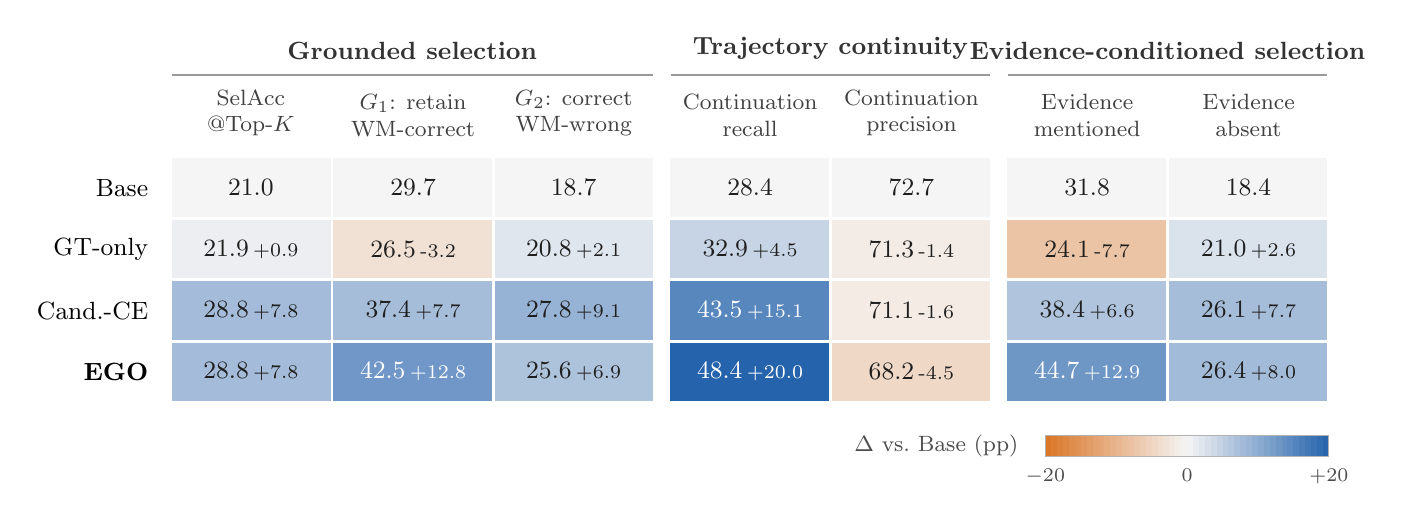
\begin{tikzpicture}[x=1cm,y=1cm,font=\small]
  % Metric groups: booktabs-style spanning rules over their columns.
  \draw[black!40,line width=0.5pt] (2.62,5.46) -- (8.73,5.46);
  \node[anchor=south,font=\small\bfseries,text=black!80] at (5.67,5.54) {Grounded selection};
  \draw[black!40,line width=0.5pt] (8.95,5.46) -- (13.01,5.46);
  \node[anchor=south,font=\small\bfseries,text=black!80] at (10.98,5.54) {Trajectory continuity};
  \draw[black!40,line width=0.5pt] (13.23,5.46) -- (17.29,5.46);
  \node[anchor=south,font=\small\bfseries,text=black!80] at (15.26,5.54) {Evidence-conditioned selection};

  % Metric column headers.
  \node[anchor=south,align=center,font=\footnotesize,text=black!75] at (3.62,4.56) {SelAcc\\@Top-$K$};
  \node[anchor=south,align=center,font=\footnotesize,text=black!75] at (5.68,4.56) {$G_1$: retain\\WM-correct};
  \node[anchor=south,align=center,font=\footnotesize,text=black!75] at (7.72,4.56) {$G_2$: correct\\WM-wrong};
  \node[anchor=south,align=center,font=\footnotesize,text=black!75] at (9.96,4.56) {Continuation\\recall};
  \node[anchor=south,align=center,font=\footnotesize,text=black!75] at (12.01,4.56) {Continuation\\precision};
  \node[anchor=south,align=center,font=\footnotesize,text=black!75] at (14.24,4.56) {Evidence\\mentioned};
  \node[anchor=south,align=center,font=\footnotesize,text=black!75] at (16.29,4.56) {Evidence\\absent};

  % Training conditions (rows); the final model is set in bold.
  \node[anchor=east,font=\small] at (2.44,4.03) {Base};
  \node[anchor=east,font=\small] at (2.44,3.25) {GT-only};
  \node[anchor=east,font=\small] at (2.44,2.47) {Cand.-CE};
  \node[anchor=east,font=\small\bfseries] at (2.44,1.69) {\method{}};

  % Cells: raw percentage, signed change from Base, and the Delta-encoded fill.
  \filldraw[fill={rgb,255:red,245;green,245;blue,245},draw=white,line width=1pt]
    (2.60,3.64) rectangle (4.65,4.42);
  \node[font=\small,text=black!88] at (3.62,4.03) {21.0};
  \filldraw[fill={rgb,255:red,236;green,238;blue,242},draw=white,line width=1pt]
    (2.60,2.86) rectangle (4.65,3.64);
  \node[font=\small,text=black!88] at (3.62,3.25) {21.9\,{\scriptsize +0.9}};
  \filldraw[fill={rgb,255:red,164;green,188;blue,217},draw=white,line width=1pt]
    (2.60,2.08) rectangle (4.65,2.86);
  \node[font=\small,text=black!88] at (3.62,2.47) {28.8\,{\scriptsize +7.8}};
  \filldraw[fill={rgb,255:red,164;green,188;blue,217},draw=white,line width=1pt]
    (2.60,1.30) rectangle (4.65,2.08);
  \node[font=\small,text=black!88] at (3.62,1.69) {28.8\,{\scriptsize +7.8}};
  \filldraw[fill={rgb,255:red,245;green,245;blue,245},draw=white,line width=1pt]
    (4.65,3.64) rectangle (6.70,4.42);
  \node[font=\small,text=black!88] at (5.68,4.03) {29.7};
  \filldraw[fill={rgb,255:red,241;green,224;blue,212},draw=white,line width=1pt]
    (4.65,2.86) rectangle (6.70,3.64);
  \node[font=\small,text=black!88] at (5.68,3.25) {26.5\,{\scriptsize -3.2}};
  \filldraw[fill={rgb,255:red,165;green,189;blue,217},draw=white,line width=1pt]
    (4.65,2.08) rectangle (6.70,2.86);
  \node[font=\small,text=black!88] at (5.68,2.47) {37.4\,{\scriptsize +7.7}};
  \filldraw[fill={rgb,255:red,112;green,151;blue,199},draw=white,line width=1pt]
    (4.65,1.30) rectangle (6.70,2.08);
  \node[font=\small,text=white] at (5.68,1.69) {42.5\,{\scriptsize +12.8}};
  \filldraw[fill={rgb,255:red,245;green,245;blue,245},draw=white,line width=1pt]
    (6.70,3.64) rectangle (8.75,4.42);
  \node[font=\small,text=black!88] at (7.72,4.03) {18.7};
  \filldraw[fill={rgb,255:red,223;green,230;blue,237},draw=white,line width=1pt]
    (6.70,2.86) rectangle (8.75,3.64);
  \node[font=\small,text=black!88] at (7.72,3.25) {20.8\,{\scriptsize +2.1}};
  \filldraw[fill={rgb,255:red,150;green,178;blue,212},draw=white,line width=1pt]
    (6.70,2.08) rectangle (8.75,2.86);
  \node[font=\small,text=black!88] at (7.72,2.47) {27.8\,{\scriptsize +9.1}};
  \filldraw[fill={rgb,255:red,173;green,195;blue,220},draw=white,line width=1pt]
    (6.70,1.30) rectangle (8.75,2.08);
  \node[font=\small,text=black!88] at (7.72,1.69) {25.6\,{\scriptsize +6.9}};
  \filldraw[fill={rgb,255:red,245;green,245;blue,245},draw=white,line width=1pt]
    (8.93,3.64) rectangle (10.98,4.42);
  \node[font=\small,text=black!88] at (9.96,4.03) {28.4};
  \filldraw[fill={rgb,255:red,198;green,212;blue,229},draw=white,line width=1pt]
    (8.93,2.86) rectangle (10.98,3.64);
  \node[font=\small,text=black!88] at (9.96,3.25) {32.9\,{\scriptsize +4.5}};
  \filldraw[fill={rgb,255:red,88;green,135;blue,190},draw=white,line width=1pt]
    (8.93,2.08) rectangle (10.98,2.86);
  \node[font=\small,text=white] at (9.96,2.47) {43.5\,{\scriptsize +15.1}};
  \filldraw[fill={rgb,255:red,37;green,99;blue,173},draw=white,line width=1pt]
    (8.93,1.30) rectangle (10.98,2.08);
  \node[font=\small,text=white] at (9.96,1.69) {48.4\,{\scriptsize +20.0}};
  \filldraw[fill={rgb,255:red,245;green,245;blue,245},draw=white,line width=1pt]
    (10.98,3.64) rectangle (13.03,4.42);
  \node[font=\small,text=black!88] at (12.01,4.03) {72.7};
  \filldraw[fill={rgb,255:red,243;green,236;blue,230},draw=white,line width=1pt]
    (10.98,2.86) rectangle (13.03,3.64);
  \node[font=\small,text=black!88] at (12.01,3.25) {71.3\,{\scriptsize -1.4}};
  \filldraw[fill={rgb,255:red,243;green,235;blue,228},draw=white,line width=1pt]
    (10.98,2.08) rectangle (13.03,2.86);
  \node[font=\small,text=black!88] at (12.01,2.47) {71.1\,{\scriptsize -1.6}};
  \filldraw[fill={rgb,255:red,239;green,216;blue,198},draw=white,line width=1pt]
    (10.98,1.30) rectangle (13.03,2.08);
  \node[font=\small,text=black!88] at (12.01,1.69) {68.2\,{\scriptsize -4.5}};
  \filldraw[fill={rgb,255:red,245;green,245;blue,245},draw=white,line width=1pt]
    (13.21,3.64) rectangle (15.26,4.42);
  \node[font=\small,text=black!88] at (14.24,4.03) {31.8};
  \filldraw[fill={rgb,255:red,235;green,196;blue,165},draw=white,line width=1pt]
    (13.21,2.86) rectangle (15.26,3.64);
  \node[font=\small,text=black!88] at (14.24,3.25) {24.1\,{\scriptsize -7.7}};
  \filldraw[fill={rgb,255:red,176;green,197;blue,221},draw=white,line width=1pt]
    (13.21,2.08) rectangle (15.26,2.86);
  \node[font=\small,text=black!88] at (14.24,2.47) {38.4\,{\scriptsize +6.6}};
  \filldraw[fill={rgb,255:red,111;green,151;blue,198},draw=white,line width=1pt]
    (13.21,1.30) rectangle (15.26,2.08);
  \node[font=\small,text=white] at (14.24,1.69) {44.7\,{\scriptsize +12.9}};
  \filldraw[fill={rgb,255:red,245;green,245;blue,245},draw=white,line width=1pt]
    (15.26,3.64) rectangle (17.31,4.42);
  \node[font=\small,text=black!88] at (16.29,4.03) {18.4};
  \filldraw[fill={rgb,255:red,218;green,226;blue,236},draw=white,line width=1pt]
    (15.26,2.86) rectangle (17.31,3.64);
  \node[font=\small,text=black!88] at (16.29,3.25) {21.0\,{\scriptsize +2.6}};
  \filldraw[fill={rgb,255:red,165;green,189;blue,217},draw=white,line width=1pt]
    (15.26,2.08) rectangle (17.31,2.86);
  \node[font=\small,text=black!88] at (16.29,2.47) {26.1\,{\scriptsize +7.7}};
  \filldraw[fill={rgb,255:red,162;green,187;blue,216},draw=white,line width=1pt]
    (15.26,1.30) rectangle (17.31,2.08);
  \node[font=\small,text=black!88] at (16.29,1.69) {26.4\,{\scriptsize +8.0}};

  % Continuous colorbar for the shared +/-20 pp scale.
  \fill[fill={rgb,255:red,218;green,119;blue,41}] (13.710,0.62) rectangle (13.785,0.88);
  \fill[fill={rgb,255:red,220;green,125;blue,50}] (13.785,0.62) rectangle (13.860,0.88);
  \fill[fill={rgb,255:red,221;green,130;blue,58}] (13.860,0.62) rectangle (13.935,0.88);
  \fill[fill={rgb,255:red,222;green,135;blue,67}] (13.935,0.62) rectangle (14.010,0.88);
  \fill[fill={rgb,255:red,223;green,141;blue,76}] (14.010,0.62) rectangle (14.085,0.88);
  \fill[fill={rgb,255:red,224;green,146;blue,84}] (14.085,0.62) rectangle (14.160,0.88);
  \fill[fill={rgb,255:red,225;green,151;blue,93}] (14.160,0.62) rectangle (14.235,0.88);
  \fill[fill={rgb,255:red,226;green,157;blue,102}] (14.235,0.62) rectangle (14.310,0.88);
  \fill[fill={rgb,255:red,227;green,162;blue,111}] (14.310,0.62) rectangle (14.385,0.88);
  \fill[fill={rgb,255:red,229;green,167;blue,119}] (14.385,0.62) rectangle (14.460,0.88);
  \fill[fill={rgb,255:red,230;green,173;blue,128}] (14.460,0.62) rectangle (14.535,0.88);
  \fill[fill={rgb,255:red,231;green,178;blue,137}] (14.535,0.62) rectangle (14.610,0.88);
  \fill[fill={rgb,255:red,232;green,183;blue,145}] (14.610,0.62) rectangle (14.685,0.88);
  \fill[fill={rgb,255:red,233;green,189;blue,154}] (14.685,0.62) rectangle (14.760,0.88);
  \fill[fill={rgb,255:red,234;green,194;blue,163}] (14.760,0.62) rectangle (14.835,0.88);
  \fill[fill={rgb,255:red,235;green,200;blue,171}] (14.835,0.62) rectangle (14.910,0.88);
  \fill[fill={rgb,255:red,236;green,205;blue,180}] (14.910,0.62) rectangle (14.985,0.88);
  \fill[fill={rgb,255:red,238;green,210;blue,189}] (14.985,0.62) rectangle (15.060,0.88);
  \fill[fill={rgb,255:red,239;green,216;blue,197}] (15.060,0.62) rectangle (15.135,0.88);
  \fill[fill={rgb,255:red,240;green,221;blue,206}] (15.135,0.62) rectangle (15.210,0.88);
  \fill[fill={rgb,255:red,241;green,226;blue,215}] (15.210,0.62) rectangle (15.285,0.88);
  \fill[fill={rgb,255:red,242;green,232;blue,223}] (15.285,0.62) rectangle (15.360,0.88);
  \fill[fill={rgb,255:red,243;green,237;blue,232}] (15.360,0.62) rectangle (15.435,0.88);
  \fill[fill={rgb,255:red,244;green,242;blue,241}] (15.435,0.62) rectangle (15.510,0.88);
  \fill[fill={rgb,255:red,241;green,242;blue,243}] (15.510,0.62) rectangle (15.585,0.88);
  \fill[fill={rgb,255:red,232;green,236;blue,240}] (15.585,0.62) rectangle (15.660,0.88);
  \fill[fill={rgb,255:red,223;green,230;blue,237}] (15.660,0.62) rectangle (15.735,0.88);
  \fill[fill={rgb,255:red,215;green,224;blue,234}] (15.735,0.62) rectangle (15.810,0.88);
  \fill[fill={rgb,255:red,206;green,218;blue,231}] (15.810,0.62) rectangle (15.885,0.88);
  \fill[fill={rgb,255:red,197;green,211;blue,228}] (15.885,0.62) rectangle (15.960,0.88);
  \fill[fill={rgb,255:red,189;green,205;blue,225}] (15.960,0.62) rectangle (16.035,0.88);
  \fill[fill={rgb,255:red,180;green,199;blue,222}] (16.035,0.62) rectangle (16.110,0.88);
  \fill[fill={rgb,255:red,171;green,193;blue,219}] (16.110,0.62) rectangle (16.185,0.88);
  \fill[fill={rgb,255:red,163;green,187;blue,216}] (16.185,0.62) rectangle (16.260,0.88);
  \fill[fill={rgb,255:red,154;green,181;blue,213}] (16.260,0.62) rectangle (16.335,0.88);
  \fill[fill={rgb,255:red,145;green,175;blue,210}] (16.335,0.62) rectangle (16.410,0.88);
  \fill[fill={rgb,255:red,137;green,169;blue,207}] (16.410,0.62) rectangle (16.485,0.88);
  \fill[fill={rgb,255:red,128;green,163;blue,204}] (16.485,0.62) rectangle (16.560,0.88);
  \fill[fill={rgb,255:red,119;green,157;blue,201}] (16.560,0.62) rectangle (16.635,0.88);
  \fill[fill={rgb,255:red,111;green,151;blue,198}] (16.635,0.62) rectangle (16.710,0.88);
  \fill[fill={rgb,255:red,102;green,144;blue,195}] (16.710,0.62) rectangle (16.785,0.88);
  \fill[fill={rgb,255:red,93;green,138;blue,192}] (16.785,0.62) rectangle (16.860,0.88);
  \fill[fill={rgb,255:red,84;green,132;blue,189}] (16.860,0.62) rectangle (16.935,0.88);
  \fill[fill={rgb,255:red,76;green,126;blue,186}] (16.935,0.62) rectangle (17.010,0.88);
  \fill[fill={rgb,255:red,67;green,120;blue,183}] (17.010,0.62) rectangle (17.085,0.88);
  \fill[fill={rgb,255:red,58;green,114;blue,180}] (17.085,0.62) rectangle (17.160,0.88);
  \fill[fill={rgb,255:red,50;green,108;blue,177}] (17.160,0.62) rectangle (17.235,0.88);
  \fill[fill={rgb,255:red,41;green,102;blue,174}] (17.235,0.62) rectangle (17.310,0.88);
  \draw[black!30,line width=0.4pt] (13.71,0.62) rectangle (17.31,0.88);
  \node[anchor=north,font=\scriptsize,text=black!70] at (13.71,0.58) {$-20$};
  \node[anchor=north,font=\scriptsize,text=black!70] at (15.51,0.58) {$0$};
  \node[anchor=north,font=\scriptsize,text=black!70] at (17.31,0.58) {$+20$};
  \node[anchor=east,font=\footnotesize,text=black!70] at (13.49,0.75) {$\Delta$ vs.\ Base (pp)};
\end{tikzpicture}
\caption{\textbf{Capability profile across controlled training conditions.}
Each cell reports the raw percentage on the common covered set
(\obs{$n{=}1{,}000$}), followed by its signed change from the Base row.  Color
encodes that change on a shared $\pm20$-percentage-point diverging scale (blue
above Base, orange below), so saturation is proportional to effect size.
Candidate alignment gains broadly in grounded selection and continuation
recall, whereas answer-only supervision (GT-only) does not.  \method{}
strengthens retention and continuation recovery further, but not on every
axis.  The evidence-conditioned columns are descriptive associations, not
interventions.}
\label{fig:capability}
\end{figure*}


\subsubsection{Where the Gain Appears: A Capability Profile}
\label{sec:er-axes}

Aggregate accuracy does not reveal whether a policy preserves a correct
world-model prior or repairs an incorrect one.  We therefore separate
$G_1$ retention from $G_2$ correction (Figure~\ref{fig:capability};
Table~\ref{tab:capability}).  Candidate alignment improves both, whereas
answer-only supervision weakens retention while offering little correction.
The final \method{} model shifts the profile further toward retaining valid
priors without uniformly improving correction.  Thus, providing a candidate
boundary at inference is insufficient: training must teach the policy when
to trust its leading hypothesis and when trajectory context warrants an
override.  The decomposition also prevents the aggregate gain from being
attributed to a single easy subset.

\begin{table*}[t]
\centering
\small
\setlength{\tabcolsep}{7pt}
\begin{tabular}{p{0.27\textwidth}p{0.66\textwidth}}
\toprule
Metric & What it tests \\
\midrule
SelAcc@Top-$K$
  & Whether the policy selects the ground-truth action from the shuffled
    world-model Top-$K$ candidate set when scores and ranks are hidden. \\
$G_1$: retain WM-correct
  & Whether the policy preserves a valid predictive prior when the
    world-model Top-$1$ action is correct. \\
$G_2$: correct WM-wrong
  & Whether the policy overrides an incorrect world-model Top-$1$ prediction
    and reselects the covered ground-truth action. \\
Continuation recall
  & Whether the policy recovers the target when it continues the immediately
    preceding behavior in the trajectory. \\
Continuation precision
  & Whether a predicted continuation is correct; this controls for an
    indiscriminate tendency to repeat the previous action. \\
Evidence-conditioned accuracy
  & Whether explicitly represented prior-action evidence separates correct
    from incorrect selections.  This is a descriptive diagnostic, not an
    intervention. \\
\bottomrule
\end{tabular}
\caption{\textbf{Operational definition of the reported capability axes.}
The metrics isolate selection, predictive-prior retention, error correction,
trajectory continuity, and evidence--decision coupling.  Their corresponding
measurements are consolidated in Figure~\ref{fig:capability}.}
\label{tab:capability}
\end{table*}


Trajectory continuity exhibits the same structure.  Candidate alignment
recovers substantially more true continuations, and the final \method{} model
achieves the strongest continuation recall.  Precision remains broadly stable
across conditions, so the recall gain is not explained by a looser tendency
to repeat the previous action.  Instead, training appears to improve access
to an already reliable temporal cue.

\subsubsection{Causal Test: The Learned Advantage Is Carried by History}
\label{sec:er-history}

We next remove completed-action history while holding the observation,
candidate set, and model fixed.  Candidate alignment loses
\obs{$10.1\pp$} (\obs{$95\%$ CI $[+6.8,+13.3]$}), and its advantage over
both controls disappears.  The replay-stage model shows the same qualitative
dependence, although this intervention was not repeated after grounding
oversampling.  A better static action prior would survive removal of history;
the observed collapse instead identifies trajectory use as the source of the
candidate-alignment gain.  This is the strongest evidence that the policy
interprets the world-model boundary conditionally rather than merely adopting
a different answer frequency.

\subsubsection{Useful Evidence, Not More Evidence}
\label{sec:er-evidence}

We finally ask whether a generated trace contains decision-relevant state or
only persuasive wording.  Answer-only supervision makes prior-action language
more frequent but less predictive of correctness.  Candidate alignment
preserves a strong association between cited temporal evidence and successful
selection, while the final \method{} model uses such language more selectively
and with the highest conditional utility (Figure~\ref{fig:capability}).  The
relevant distinction is therefore not whether a model \emph{says} that it used
history, but whether the represented evidence discriminates correct from
incorrect decisions.  Because this split is observational, it motivates—but
does not replace—the paired interventions below.

The belief channel provides a complementary control.  Answer-only
supervision often collapses belief into an action copy, whereas candidate
alignment and the final \method{} model largely avoid this failure mode.
For the candidate-aligned policy, replacing only the belief while holding
reasoning fixed yields a paraphrase-adjusted action-flip rate of
\obs{$9.3\%$}.  Low echo and nonzero interventional sensitivity together show
that the belief field can carry decision-relevant state without simply
restating the answer.  This causal interpretation applies to the evaluated
candidate-aligned policy only; the final model lacks the corresponding
intervention.  Table~\ref{tab:trace-echo} makes the contrast visible in one
controlled trace comparison.

% Reserve Table 2 for additional quantitative diagnostics.
\addtocounter{table}{1}
\begin{table*}[t]
\footnotesize
\setlength{\parindent}{0pt}
\textbf{Cooking anticipation case.} Observation interval
\obs{$3620.4$--$3628.4$}\,s; target time \obs{$3631.0$}\,s; \obs{$122$}
completed actions in the available history.\par
\smallskip
\textbf{WM candidate set} (shuffled; scores and ranks hidden from the policy):
check heat (GT, WM rank \obs{$3$}) \textperiodcentered{} flip flatbread
\textperiodcentered{} transfer flatbread \textperiodcentered{} cook flatbread
\textperiodcentered{} press dough \textperiodcentered{} roll dough
\textperiodcentered{} knead dough (WM rank \obs{$1$}) \textperiodcentered{}
sprinkle flour \textperiodcentered{} shape dough \textperiodcentered{} cut
dough.\par
\smallskip
\textbf{Completed-action history} (last \obs{$8$}): \ldots{} $\rightarrow$ roll
dough $\rightarrow$ flip ingredient $\rightarrow$ check heat $\rightarrow$ roll
dough $\rightarrow$ check heat $\rightarrow$ flip ingredient $\rightarrow$ press
dough $\rightarrow$ cook flatbread.\par
\medskip
\setlength{\tabcolsep}{6pt}
\begin{tabular}{@{}p{0.115\textwidth}p{0.845\textwidth}@{}}
\toprule
Model & reasoning $\rightarrow$ belief $\rightarrow$ action \\
\midrule
Base
  & \emph{``The current frame \textsc{shows} the flatbread being cooked on the
    hot surface, and the person's hand is positioned to flip it\ldots{}
    Flipping the flatbread is the logical next step to ensure even cooking.''}
    \newline
    \textsc{belief} --- Flipping the flatbread to cook the other side.
    \newline
    $\rightarrow$ \textbf{flip flatbread} $\times$
    \quad{\scriptsize[scene description via ``shows'']} \\
GT-only
  & \emph{``The current frame \textsc{shows} the flatbread being cooked on the
    hot surface\ldots{} The most logical next step, given the context of
    cooking flatbread, is to flip it\ldots{} This aligns with
    \underline{the previous actions} of checking heat and flipping the
    flatbread.''}
    \newline
    \textsc{belief} --- \textbf{flip flatbread}
    \quad{\scriptsize[action-copying belief]}
    \newline
    $\rightarrow$ \textbf{flip flatbread} $\times$
    \quad{\scriptsize[scene description via ``shows'']} \\
Cand.-CE
  & \emph{``The current frame \textsc{shows} the flatbread being cooked on the
    hot surface, and \underline{the previous action} was flipping the
    ingredient. The next logical step is to continue cooking the flatbread, as
    it is still on the fire and needs to be cooked through.''}
    \newline
    \textsc{belief} --- Cook the flatbread on the fire.
    \newline
    $\rightarrow$ \textbf{cook flatbread} $\times$
    \quad{\scriptsize[scene description via ``shows'']} \\
\method{}
  & \emph{``\textbf{I have just finished pressing the dough and am now
    observing the fire to assess the heat for cooking. The flames are visible
    and active, indicating the stove is ready.} I need to ensure the heat is
    suitable before proceeding with the next step in cooking.''}
    \newline
    \textsc{belief} --- I am in the middle of assessing the heat level for
    cooking the flatbread.
    \newline
    $\rightarrow$ \textbf{check heat} \cmark
    \quad{\scriptsize[state-bearing belief; no explicit prior-action reference]} \\
\bottomrule
\end{tabular}
\caption{\textbf{A state-bearing belief enables correction when an
action-copying belief does not.}  The four evaluated policies receive the
same observation, completed-action history, shuffled candidate set, and
prompt.  Generated traces are reproduced verbatim, with \ldots{} marking
omitted text.  To avoid anecdotal selection, we apply a fixed criterion to the
common covered set: all four traces must be valid, GT-only must copy its chosen
action into the belief field and answer incorrectly, and \method{} must answer
correctly.  This criterion identifies \obs{$31$} of \obs{$915$} points; the
example shown is one of the \obs{$18$} for which Cand.-CE is also incorrect.
\underline{Underlined} spans explicitly reference prior actions under the
same rule used for the mention-rate analysis, whereas \textbf{bold} spans
express the model's current task state.}
\label{tab:trace-echo}
\end{table*}

\subsubsection{What Is and Is Not Established}
\label{sec:er-scope}

The current same-cohort evidence establishes three claims.  First,
candidate-constrained training improves selection beyond both the
world-model Top-\obs{$1$} policy and answer-only supervision.  Second, the
improvement appears in both retention and correction rather than in a single
easy subset.  Third, the gain is causally dependent on completed-action
history.  Together these results support the paper's modular account:
the world model defines a visually grounded action boundary, while the
language policy learns to interpret task and trajectory context within that
boundary.

The final training stage augments Retrospection-with-Replay with grounding
oversampling at a fixed optimization budget.  It restores overall selection
to the candidate-aligned level while strengthening retention, continuation
recovery, and evidence utility (Figure~\ref{fig:capability}).  However, the
preregistered \obs{$1\pp$} non-inferiority criterion is not met: the paired
SelAcc difference is \obs{$-0.64\pp$}
(\obs{$95\%$ CI $[-3.88,+2.91]$}), and correction also declines.  The interval
contains zero, so the result does not establish degradation; equally, its
lower bound is too low to establish preservation under the specified margin.
We therefore treat the final stage as a recovery of the aggregate score with
a changed capability profile, not as uniformly lossless Retrospection.

{\color{pendingred}
\paragraph{Limitation of the final-stage intervention.}
Axis 5 is not established for the final \method{} model because belief swap
was not evaluated after grounding oversampling.  At the preceding replay
stage, belief sensitivity remained below its preregistered threshold while
reasoning sensitivity was the strongest among the evaluated conditions.  This
suggests a redistribution toward the reasoning channel, but the final model's
zero belief--action echo is not an interventional substitute.  Final-stage
belief-utility diagnostics therefore remain exploratory.
\par}

{\color{pendingred}
\paragraph{Excluded proxy.}
First-person phrasing is excluded from the capability profile because it
changes sharply with prompt regime and does not positively predict correctness
within the answer-only control.  Contrastive connectives are likewise rare,
and their association with accuracy reverses across the replay and grounding
stages on a small subset.  Both are therefore treated as template-sensitive
surface forms rather than evidence of embodied reasoning; neither supports
the paper's claims.
\par}

\end{document}
